\documentclass{Alexandre}
\usepackage[portuguese, ruled, linesnumbered]{algorithm2e}
\usepackage{multirow}
\usepackage{multicol}
\usepackage{color}
\usepackage{diagbox}
\usepackage{setspace}
\usepackage{listings}
\usepackage{color}
\usepackage{caption}
\usepackage{mwe}
\usepackage[normalem]{ulem}
\usepackage[framemethod=tikz]{mdframed}

\definecolor{codegreen}{rgb}{0,0.6,0}
\definecolor{codegray}{rgb}{0.5,0.5,0.5}
\definecolor{codepurple}{rgb}{0.58,0,0.82}
\definecolor{backcolour}{rgb}{0.95,0.95,0.92}

\lstdefinestyle{mystyle}{
  backgroundcolor=\color{backcolour},   commentstyle=\color{codegreen},
  keywordstyle=\color{magenta},
  numberstyle=\tiny\color{codegray},
  stringstyle=\color{codepurple},
  basicstyle=\footnotesize,
  breakatwhitespace=false,         
  breaklines=true,
  captionpos=b,                   
  keepspaces=true,                 
  numbers=left,                    
  numbersep=5pt,                  
  showspaces=false,                
  showstringspaces=false,
  showtabs=false,                  
  tabsize=2
}

\setbeamertemplate{bibliography item}[triangle]

\title{Artigo Colaborativo}
\subtitle{iLibras}
\author{Alexandre Mendonça Fava\inst{1}}


\institute[UDESC]{
  \newline \newline \newline
  \inst{1}
  Mestrado Acadêmico em Computação Aplicada - PPGCA
}

\date{16 Agosto 2019}

\subject{}

\logo{

\includegraphics[scale=0.8]{Figuras/Logo-UDESC.jpg}
}

\begin{document}


\begin{frame}
  \titlepage
\end{frame}
%[Transparência 1] Bom dia, eu me chamo Alexandre, e nessa apresentação irei falar sobre o artigo que selecionei, o qual fala sobre o iLibras.


\begin{frame}{AGRADECIMENTOS}

    O presente trabalho foi realizado com apoio da Coordenação de Aperfeiçoamento de Pessoal de Nível Superior - Brasil (CAPES) - Código de Financiamento 001. 

\end{frame}
%[Transparência 2] Destaco que o presente trabalho sobre o iLibras foi realizado com total apoio da CAPES.


\begin{frame}{APRESENTAÇÃO}

    \begin{figure}
        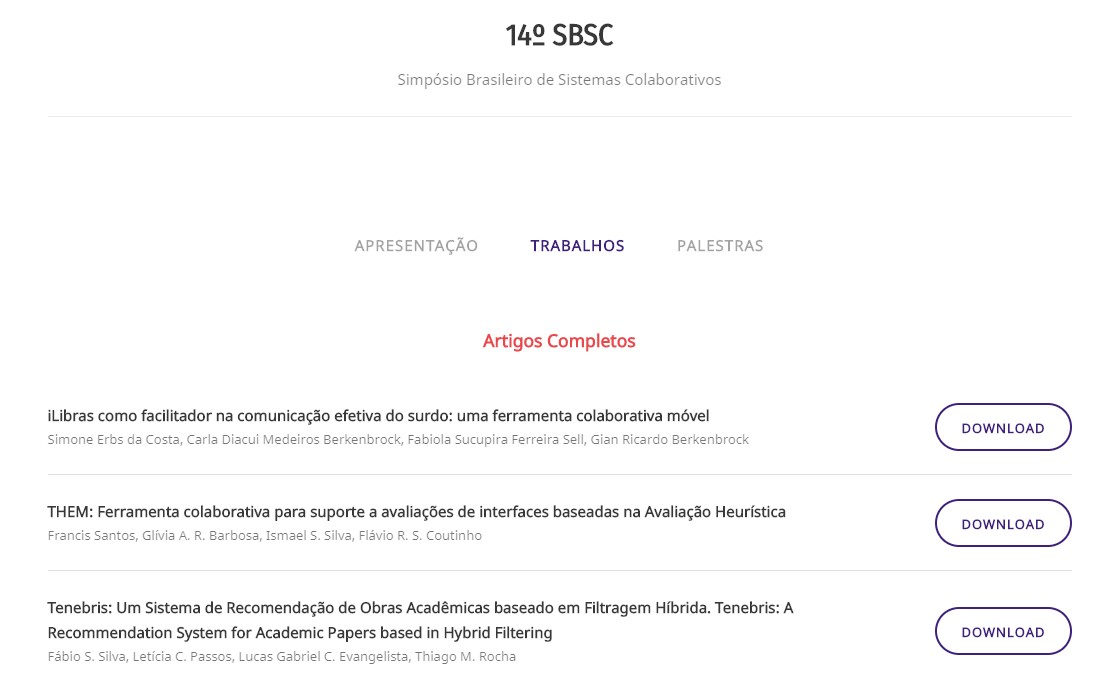
\includegraphics[scale = 0.4]{Figuras/ArtigoSBSC14.jpg}
    \end{figure}

\end{frame}
%[Transparência 3] Antes de começar, eu gostaria de esclarecer que fiquei procurando alguns artigos da SBSC, mas nenhum me agradava totalmente, até que esse iLibras me chamou atenção. Me chamou atenção mais por causa dos autores do artigo, principalmente uma tal Carla.


\begin{frame}{APRESENTAÇÃO}

    \begin{figure}
        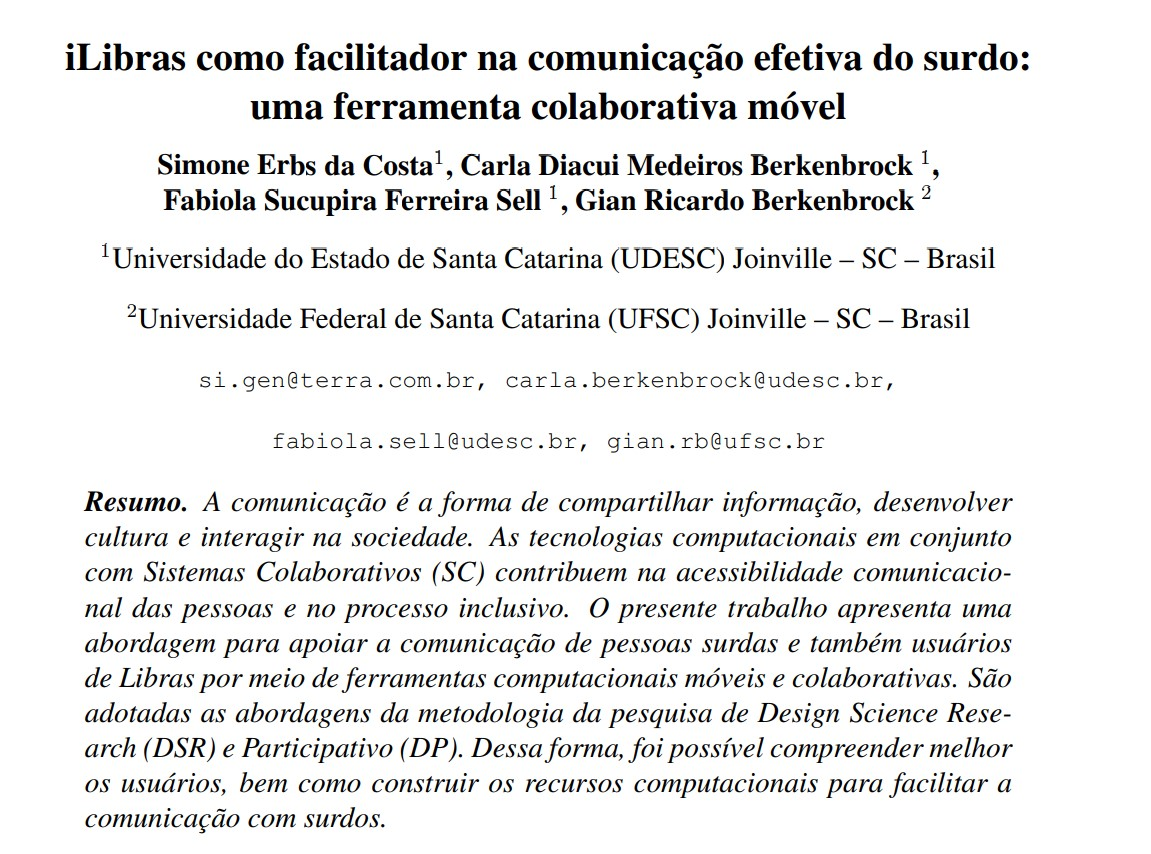
\includegraphics[scale = 0.3]{Figuras/iLibras.jpg}
    \end{figure}

\end{frame}
%[Transparência 4] Notoriamente o artigo é daqui da UDESC. E já no resumo, se pode ter uma melhor noção do que se trata o artigo. Com o artigo apresentando "uma abordagem para apoiar a comunicação de pessoas surdas e também usuários por meio de ferramenras móveis e colaborativas".


\begin{frame}{DESING SCIENCE RESEARCH}
    
    Elevar o desempenho do resultado da pesquisa dos sistemas de informação, trazendo contribuições para a comunidade científica, sendo seu paradigma orientado à solução de um ou mais problemas específicos

\end{frame}
%[Transparência 5] Nesse sentido, o artigo elenca algumas diretrizes do DESING SCIENCE RESEARCH aplicado ao artigo.


\begin{frame}{DIRETRIZES}
    
    \begin{figure}
        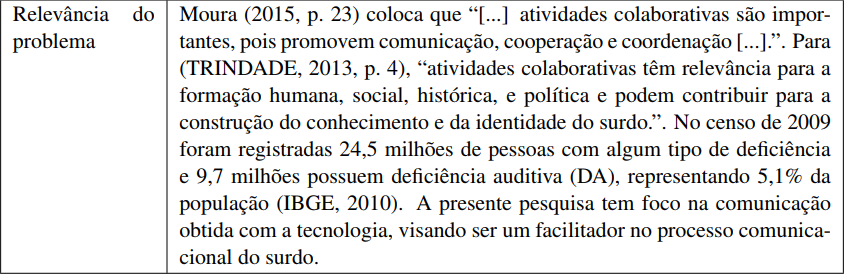
\includegraphics[scale = 0.5]{Figuras/DSR-1.png}
    \end{figure}

\end{frame}
%[Transparência 6] A primeira diretriz diz respeito a relevância do problema. É através dela que o artigo, apresenta o quanto a comunicação é importante para atividades colaborativas e apresenta o censo com os números de surdos no Brasil.


\begin{frame}{DIRETRIZES}
    
    \begin{figure}
        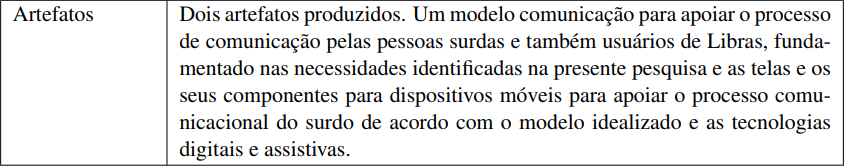
\includegraphics[scale = 0.5]{Figuras/DSR-2.png}
    \end{figure}

\end{frame}
%[Transparência 7] Nessa diretriz são apresentados os artefatos. No caso desse artigo são construidos dois:
%Um Modelo de Comunicação Efetiva (MCE)
%E o desenvolvimento de uma Comunicação Alternativa, denominado como iLibras


\begin{frame}{DIRETRIZES}
    
    \begin{figure}
        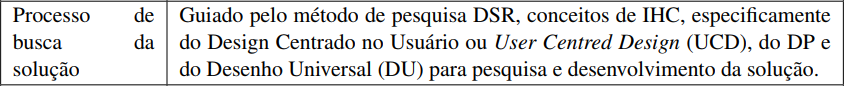
\includegraphics[scale = 0.5]{Figuras/DSR-3.png}
    \end{figure}

\end{frame}
%[Transparência 8] Aqui são informados os métodos e assuntos nos quais o estudo irá se basear para o desenvolvimento e criação dos artefatos.


\begin{frame}{DIRETRIZES}
    
    \begin{figure}
        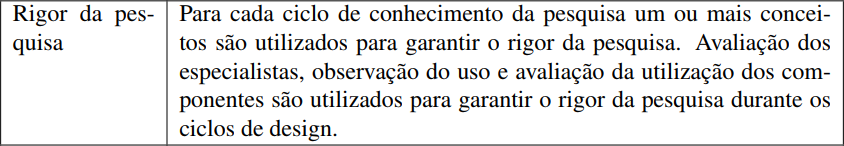
\includegraphics[scale = 0.5]{Figuras/DSR-4.png}
    \end{figure}

\end{frame}
%[Transparência 9] No rigor da pesquisa o artigo define três ciclos, sendo:
%Conhecendo o usuário
%Modelo de Comunicabilidade
%Protótipo de Comunicabilidade


\begin{frame}{DIRETRIZES}
    
    \begin{figure}
        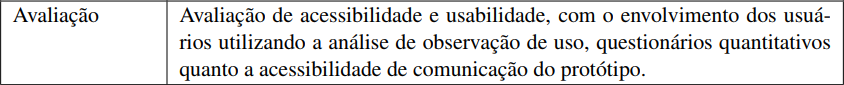
\includegraphics[scale = 0.5]{Figuras/DSR-5.png}
    \end{figure}

\end{frame}
%[Transparência 10] Na avaliação são definidos os métodos analisar a pesquisa, visando a avaliação da acessibilidade e usabilidade, como:
%Questionários
%Observação


\begin{frame}{DIRETRIZES}
    
    \begin{figure}
        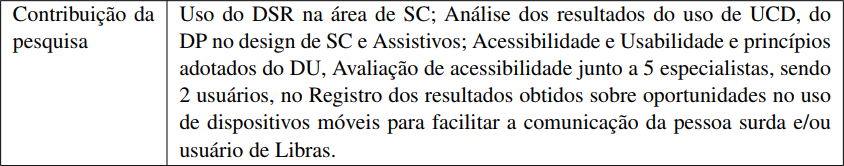
\includegraphics[scale = 0.5]{Figuras/DSR-6.png}
    \end{figure}

\end{frame}
%[Transparência 11] Dentra as constribuições desta pesquisa, está o registro dos resultados obtidos sobre as oportunidades no uso de dispositivos móveis para facilitar a comunicação das pessoas surdas.


\begin{frame}{SOFTWARE}
    
    \begin{figure}
        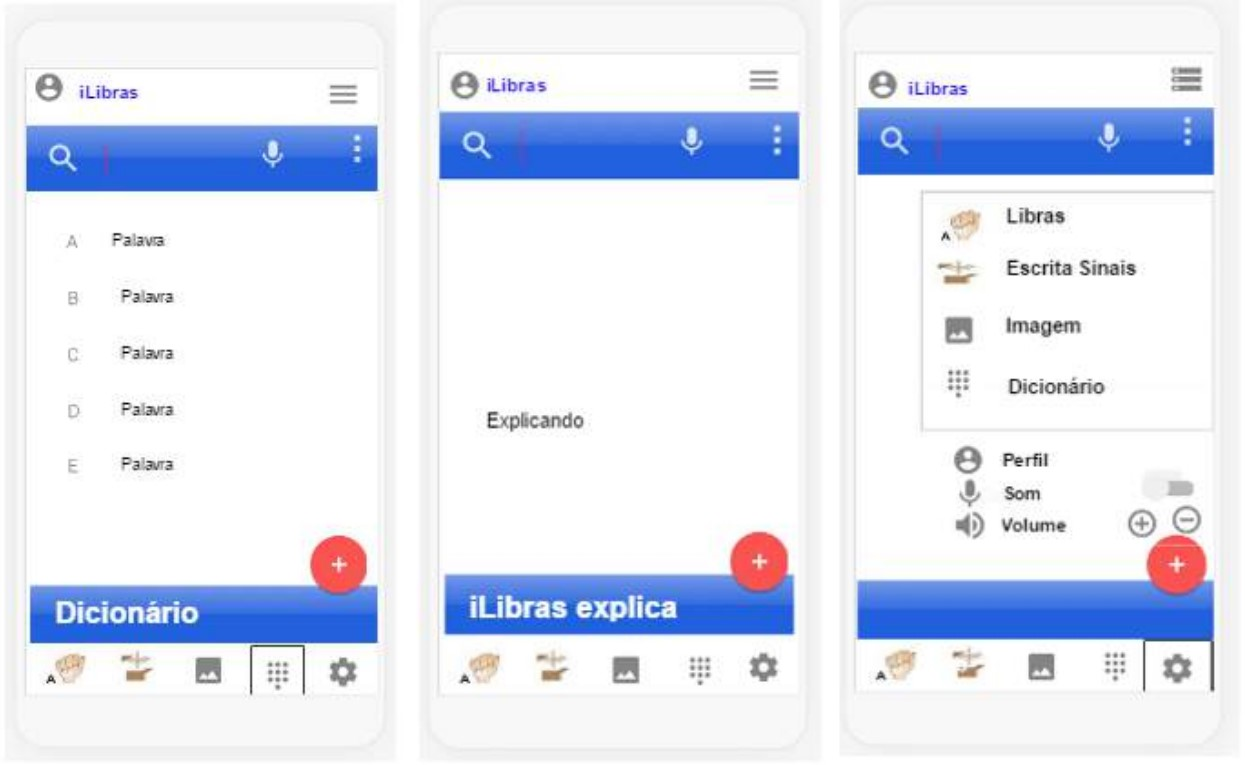
\includegraphics[scale = 0.3]{Figuras/Aplicativo.jpg}
    \end{figure}

\end{frame}
%[Transparência 12] Foi modelado e desenvolvido um dicionário de sinais multimídia que armazenará uma representação em imagem, gif ou vídeo em Libras
%A primeira tela se refere a pesquisar no dicionário de palavras.
%A segunda tela se refere a tela explicativa do aplicativo iLibras.
%A terceira tela se refere ao menu lateral que pode ser acessado de qualquer tela.


\begin{frame}{SOFTWARE}
    
    \begin{figure}
        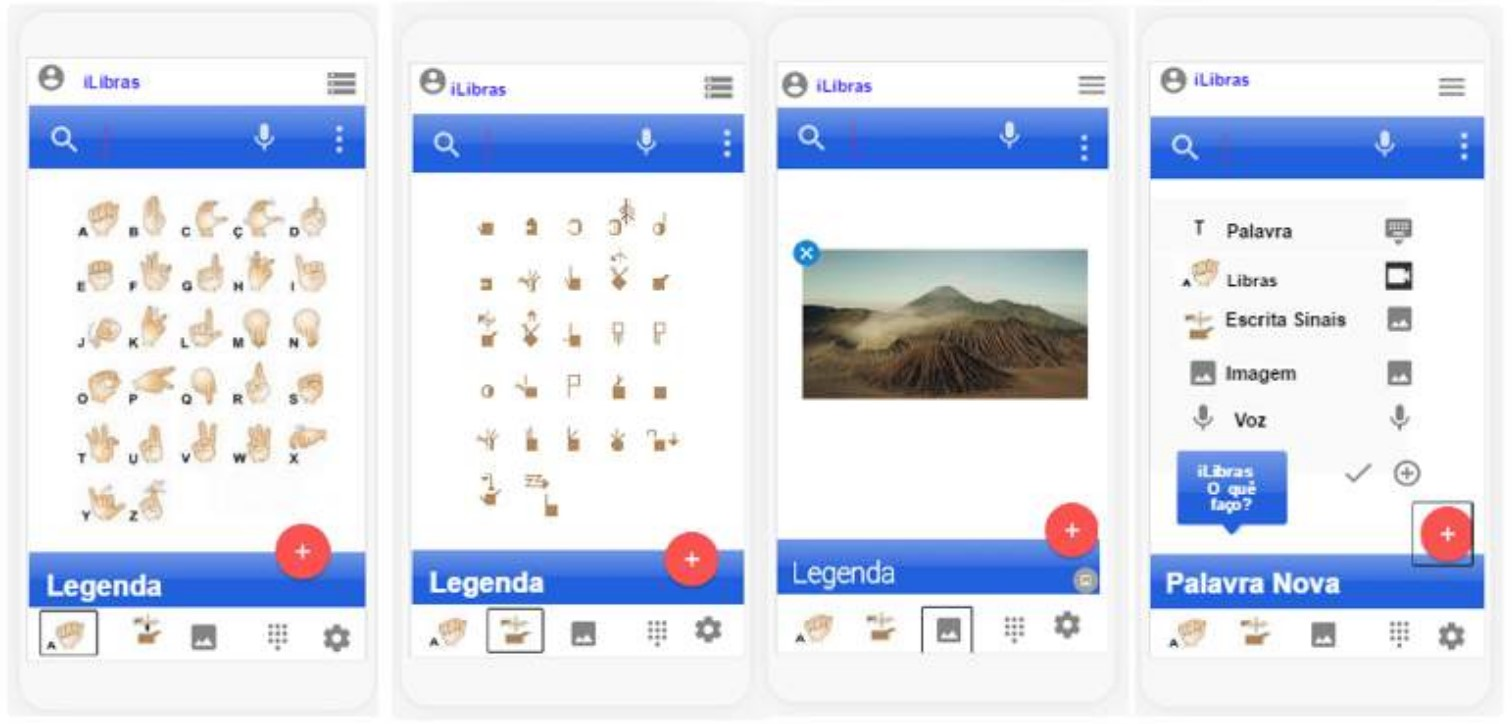
\includegraphics[scale = 0.25]{Figuras/Gestos.jpg}
    \end{figure}

\end{frame}
%[Transparência 13] O aplicativo transcreve ao usuário o conteúdo de Libras, tanto via texto, imagem, voz, ou signwriting.


\begin{frame}{RESULTADOS}
    
    \begin{figure}
        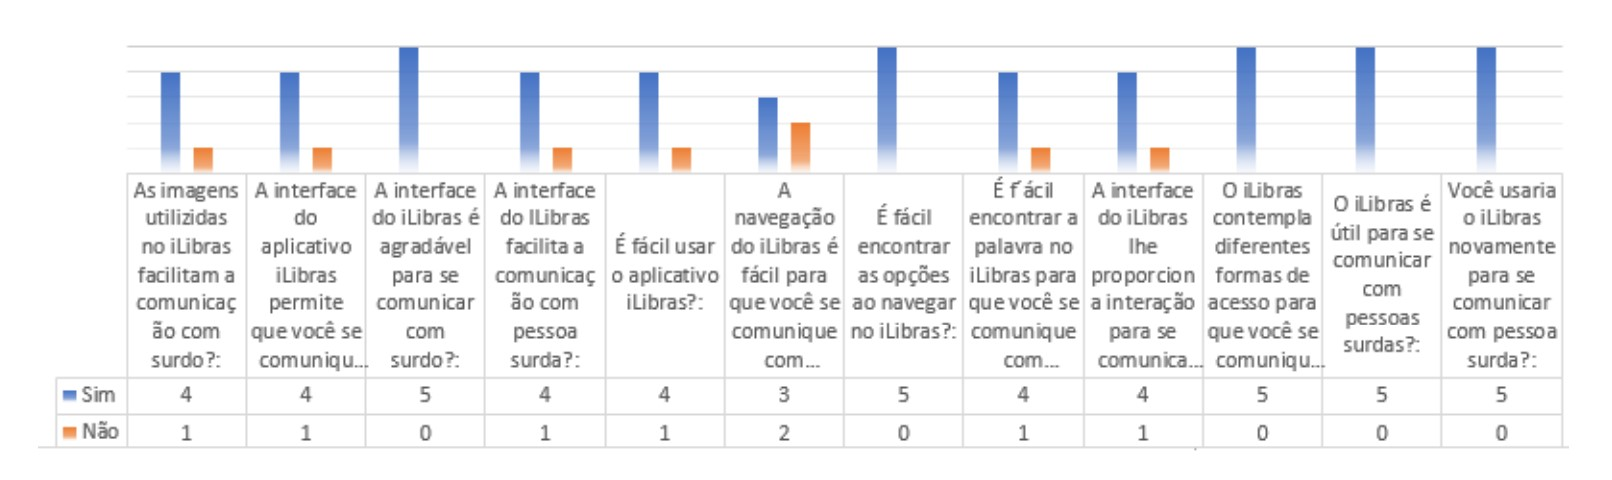
\includegraphics[scale = 0.28]{Figuras/Resultados.jpg}
    \end{figure}

\end{frame}
%[Transparência 14] Além do questionário realizado, por intermédio de emoticons com especialistas, também foi realizada uma “Entrevista Aberta".


\begin{frame}{CONCLUSÃO}
    
    \begin{itemize}
        \item Ampliação do vocabulário de estudantes surdos, surdos e ouvintes, usuários ou interessados em aprender Libras.
        \item Acessibilidade comunicacional para as pessoa com surdez e deficientes auditivas. 
    \end{itemize}

\end{frame}
%[Transparência 15] Foi desenvolvida uma aplicação para proprocionar maior acessibilidade aos surdos, no entanto o aplicativo não recebeu notas muito boas no Google Play.


\begin{frame}
    \begin{center}
        \textit{"A comunicação é a forma de compartilhar informação, desenvolver cultura e interagir na sociedade" - Simone Erbs da Costa, 2018}\\
        \vspace{1.5cm}
        \begin{Huge} 
            Obrigado!\\
        \end{Huge}
        \bigskip
        Alexandre Mendonça Fava - \alert{alexandre.fava@hotmail.com}\\
    \end{center}
\end{frame}

\end{document}